%%%%%%%%%%%%%%%%%%%%%%%%%%%%%%%%%%%%%%%%%%%%%%%%%%%%%%%%%%%%%%%
%% BRIEF VERSION OF OXFORD THESIS TEMPLATE FOR CHAPTER PREVIEWS

%%%%% CHOOSE PAGE LAYOUT
% format for PDF output (ie equal margins, no extra blank pages):
\documentclass[spanish, a4paper,nobind]{templates/ociamthesis}

% add hyperref package with links hidden %
%\usepackage[colorlinks=false,pdfpagelabels,hidelinks]{hyperref}
\usepackage[colorlinks=true,pdfpagelabels,hidelinks]{hyperref}

% add float package to allow manual control of figure positioning %
\usepackage{float}

%UL set section header spacing
\usepackage{titlesec}
% 
\titlespacing\subsubsection{0pt}{24pt plus 4pt minus 2pt}{0pt plus 2pt minus 2pt}

%%%%%%%%%%%%%
% TIPOGRAFÍA 
%%%%%%%%%%%%%
\usepackage{libertinus} % Fuente LIBERTINE Linux
%%
% UL: You can set the general paragraph spacing here - I've set it to 2pt (was 0) so
% it's less claustrophobic
%
%\setlength{\parskip}{2pt plus 1pt}

%
% UL 30 Nov 2018 pandoc puts lists in 'tightlist' command when no space between bullet points in Rmd file
\providecommand{\tightlist}{%
  \setlength{\itemsep}{0pt}\setlength{\parskip}{0pt}}
 
% UL 1 Dec 2018, fix to include code in shaded environments
\usepackage{color}
\usepackage{fancyvrb}
\newcommand{\VerbBar}{|}
\newcommand{\VERB}{\Verb[commandchars=\\\{\}]}
\DefineVerbatimEnvironment{Highlighting}{Verbatim}{commandchars=\\\{\}}
% Add ',fontsize=\small' for more characters per line
\usepackage{framed}
\definecolor{shadecolor}{RGB}{248,248,248}
\newenvironment{Shaded}{\begin{snugshade}}{\end{snugshade}}
\newcommand{\AlertTok}[1]{\textcolor[rgb]{0.94,0.16,0.16}{#1}}
\newcommand{\AnnotationTok}[1]{\textcolor[rgb]{0.56,0.35,0.01}{\textbf{\textit{#1}}}}
\newcommand{\AttributeTok}[1]{\textcolor[rgb]{0.77,0.63,0.00}{#1}}
\newcommand{\BaseNTok}[1]{\textcolor[rgb]{0.00,0.00,0.81}{#1}}
\newcommand{\BuiltInTok}[1]{#1}
\newcommand{\CharTok}[1]{\textcolor[rgb]{0.31,0.60,0.02}{#1}}
\newcommand{\CommentTok}[1]{\textcolor[rgb]{0.56,0.35,0.01}{\textit{#1}}}
\newcommand{\CommentVarTok}[1]{\textcolor[rgb]{0.56,0.35,0.01}{\textbf{\textit{#1}}}}
\newcommand{\ConstantTok}[1]{\textcolor[rgb]{0.00,0.00,0.00}{#1}}
\newcommand{\ControlFlowTok}[1]{\textcolor[rgb]{0.13,0.29,0.53}{\textbf{#1}}}
\newcommand{\DataTypeTok}[1]{\textcolor[rgb]{0.13,0.29,0.53}{#1}}
\newcommand{\DecValTok}[1]{\textcolor[rgb]{0.00,0.00,0.81}{#1}}
\newcommand{\DocumentationTok}[1]{\textcolor[rgb]{0.56,0.35,0.01}{\textbf{\textit{#1}}}}
\newcommand{\ErrorTok}[1]{\textcolor[rgb]{0.64,0.00,0.00}{\textbf{#1}}}
\newcommand{\ExtensionTok}[1]{#1}
\newcommand{\FloatTok}[1]{\textcolor[rgb]{0.00,0.00,0.81}{#1}}
\newcommand{\FunctionTok}[1]{\textcolor[rgb]{0.00,0.00,0.00}{#1}}
\newcommand{\ImportTok}[1]{#1}
\newcommand{\InformationTok}[1]{\textcolor[rgb]{0.56,0.35,0.01}{\textbf{\textit{#1}}}}
\newcommand{\KeywordTok}[1]{\textcolor[rgb]{0.13,0.29,0.53}{\textbf{#1}}}
\newcommand{\NormalTok}[1]{#1}
\newcommand{\OperatorTok}[1]{\textcolor[rgb]{0.81,0.36,0.00}{\textbf{#1}}}
\newcommand{\OtherTok}[1]{\textcolor[rgb]{0.56,0.35,0.01}{#1}}
\newcommand{\PreprocessorTok}[1]{\textcolor[rgb]{0.56,0.35,0.01}{\textit{#1}}}
\newcommand{\RegionMarkerTok}[1]{#1}
\newcommand{\SpecialCharTok}[1]{\textcolor[rgb]{0.00,0.00,0.00}{#1}}
\newcommand{\SpecialStringTok}[1]{\textcolor[rgb]{0.31,0.60,0.02}{#1}}
\newcommand{\StringTok}[1]{\textcolor[rgb]{0.31,0.60,0.02}{#1}}
\newcommand{\VariableTok}[1]{\textcolor[rgb]{0.00,0.00,0.00}{#1}}
\newcommand{\VerbatimStringTok}[1]{\textcolor[rgb]{0.31,0.60,0.02}{#1}}
\newcommand{\WarningTok}[1]{\textcolor[rgb]{0.56,0.35,0.01}{\textbf{\textit{#1}}}}

%UL 2 Dec 2018 add a bit of white space before and after code blocks
\renewenvironment{Shaded}
{
  \vspace{10pt}%
  \begin{snugshade}%
}{%
  \end{snugshade}%
  \vspace{8pt}%
}
%UL 2 Dec 2018 reduce whitespace around verbatim environments
\usepackage{etoolbox}
\makeatletter
\preto{\@verbatim}{\topsep=0pt \partopsep=0pt }
\makeatother

%UL 28 Mar 2019, enable strikethrough
\usepackage[normalem]{ulem}

%UL use soul package for correction highlighting
\usepackage{soul}
\usepackage{xcolor}
\newcommand{\ctext}[3][RGB]{%
  \begingroup
  \definecolor{hlcolor}{#1}{#2}\sethlcolor{hlcolor}%
  \hl{#3}%
  \endgroup
}
\soulregister\ref7
\soulregister\cite7
\soulregister\autocite7
\soulregister\textcite7
\soulregister\pageref7

% user-included things with header_includes or in_header will appear here
% kableExtra packages will appear here if you use library(kableExtra)
\usepackage[utf8]{inputenc}
\usepackage{graphicx}
\usepackage{lipsum}

%%%%% SELECT YOUR DRAFT OPTIONS
% Three options going on here; use in any combination.  But remember to turn the first two off before
% generating a PDF to send to the printer!

% This adds a "DRAFT" footer to every normal page.  (The first page of each chapter is not a "normal" page.)

% This highlights (in blue) corrections marked with (for words) \mccorrect{blah} or (for whole
% paragraphs) \begin{mccorrection} . . . \end{mccorrection}.  This can be useful for sending a PDF of
% your corrected thesis to your examiners for review.  Turn it off, and the blue disappears.

%%%%% BIBLIOGRAPHY SETUP
% Note that your bibliography will require some tweaking depending on your department, preferred format, etc.
% The options included below are just very basic "sciencey" and "humanitiesey" options to get started.
% If you've not used LaTeX before, I recommend reading a little about biblatex/biber and getting started with it.
% If you're already a LaTeX pro and are used to natbib or something, modify as necessary.
% Either way, you'll have to choose and configure an appropriate bibliography format...

% The science-type option: numerical in-text citation with references in order of appearance.
% \usepackage[style=numeric-comp, sorting=none, backend=biber, doi=false, isbn=false]{biblatex}
% \newcommand*{\bibtitle}{References}

% The humanities-type option: author-year in-text citation with an alphabetical works cited.
% \usepackage[style=authoryear, sorting=nyt, backend=biber, maxcitenames=2, useprefix, doi=false, isbn=false]{biblatex}
% \newcommand*{\bibtitle}{Works Cited}

%UL 3 Dec 2018: set this from YAML in index.Rmd
\usepackage[style=authoryear, sorting=nyt, backend=biber, maxcitenames=2, useprefix, doi=false, isbn=false]{biblatex}
\newcommand*{\bibtitle}{Works Cited}

% This makes the bibliography left-aligned (not 'justified') and slightly smaller font.
\renewcommand*{\bibfont}{\raggedright\small}

% Change this to the name of your .bib file (usually exported from a citation manager like Zotero or EndNote).

%%%%% YOUR OWN PERSONAL MACROS
% This is a good place to dump your own LaTeX macros as they come up.

% To make text superscripts shortcuts
	\renewcommand{\th}{\textsuperscript{th}} % ex: I won 4\th place
	\newcommand{\nd}{\textsuperscript{nd}}
	\renewcommand{\st}{\textsuperscript{st}}
	\newcommand{\rd}{\textsuperscript{rd}}

%%%%%%% PAGE HEADERS AND FOOTERS %%%%%%%%%
\usepackage{fancyhdr}
\setlength{\headheight}{15pt}
%\fancyhf{} % limpamos encabezados e pés de páxima
\pagestyle{fancy} % activa encabezados
\renewcommand{\chaptermark}[1]{\markboth{\thechapter. #1}{\thechapter. #1}} % marca capítulos
\renewcommand{\sectionmark}[1]{\markright{\thesection. #1}{\thesection. #1}} % marca seccións
\renewcommand{\headrulewidth}{0.5pt} % liña baixo encabezados
%%%

%%%%% THE ACTUAL DOCUMENT STARTS HERE
\begin{document}
%%%%% CHOOSE YOUR LINE SPACING HERE
% This is the official option.  Use it for your submission copy and library copy:
%\setlength{\textbaselineskip}{22pt plus2pt}
% This is closer spacing (about 1.5-spaced) that you might prefer for your personal copies:
%\setlength{\textbaselineskip}{18pt plus2pt minus1pt} % interliñado 1.5
\setlength{\textbaselineskip}{16pt plus2pt minus1pt} % interliñado 1.25
% UL: You can set the general paragraph spacing here - I've set it to 2pt (was 0) so
% it's less claustrophobic
\setlength{\parskip}{2pt plus 1pt}

% Leave this line alone; it gets things started for the real document.
\setlength{\baselineskip}{\textbaselineskip}

% all your chapters and appendices will appear here
\hypertarget{conceptos-sobre-a-monodia-medieval}{%
\chapter*{Conceptos sobre a monodia medieval}\label{conceptos-sobre-a-monodia-medieval}}
\addcontentsline{toc}{chapter}{Conceptos sobre a monodia medieval}

\minitoc

\hypertarget{os-sistemas-modais}{%
\section*{Os sistemas modais}\label{os-sistemas-modais}}
\addcontentsline{toc}{section}{Os sistemas modais}

\hypertarget{concepto-de-modo}{%
\subsection*{Concepto de modo}\label{concepto-de-modo}}
\addcontentsline{toc}{subsection}{Concepto de modo}

\begin{itemize}
\item
  \textbf{Modalidade}. A modalidade é un sistema de organización musical baseado nos intervalos. Este concepto está relacionado especialmente coa \emph{melodía}, se temos en conta que esta é unha sucesión ordenada de intervalos.
\item
  \textbf{Modo}. Nos sistemas modais, o concepto básico é o \textbf{de modo}. Consiste na organización dos intervalos en grupos nos que certas notas teñen unha importancia especial.
\end{itemize}

\hypertarget{organizaciuxf3n-do-modo}{%
\subsection*{Organización do modo}\label{organizaciuxf3n-do-modo}}
\addcontentsline{toc}{subsection}{Organización do modo}

Os modos, baséanse en pequenos grupos de notas que abarcan en total un intervalo de cuarta ou quinta (ás veces terceira). Entre as dúas notas extremas sitúanse outras que dividen o conxunto en pequenos intervalos, que non teñen por que axustarse necesariamente a tonos ou ao semitonos.

\begin{figure}
\centering
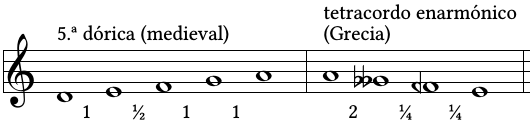
\includegraphics{figures/ud-03/grupos.png}
\caption{Grupos}
\end{figure}

Estes pequenos grupos únense a outros, ben utilizando as notas extremas como notas comúns, ou ben cunha certa separación entre ambos (habitualmente dun tono). Este conxunto de dúas ou máis unidades, dá lugar ao ámbito completo do modo, que pode ser dunha oitava ou maior.

\begin{figure}
\centering
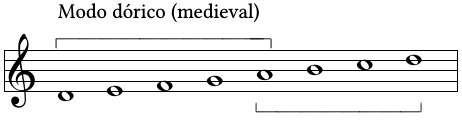
\includegraphics{figures/ud-03/escalas-2.png}
\caption{Modo dórico}
\end{figure}

\hypertarget{o-ritmo-nos-sistemas-modais}{%
\subsection*{O ritmo nos sistemas modais}\label{o-ritmo-nos-sistemas-modais}}
\addcontentsline{toc}{subsection}{O ritmo nos sistemas modais}

As definicións antigas da música facían referencia á arte (ou a ciencia) \emph{de medir ben}. Esta medida debíase facer en dúas dimensións: na da \textbf{altura} dos sons, entoando correctamente os intervalos; e na da \textbf{duración} dos sons, levando adecuadamente o ritmo. Ámbalas dimensións definen a \emph{melodía}, que é o elemento fundamental nas músicas modais.

\hypertarget{tipos-de-ritmo}{%
\subsubsection*{Tipos de ritmo}\label{tipos-de-ritmo}}
\addcontentsline{toc}{subsubsection}{Tipos de ritmo}

Consideramos dous estilos fundamentais de ritmo:

\begin{itemize}
\item
  Ritmo \textbf{libre}:

  As duracións dos sons non se axustan a ningún pulso, podendo alongarse ou acurtarse a vontade dos intérpretes. Na música vocal, o ritmo adoita axustarse ás necesidades do texto. Denomínaselle ás veces \textbf{ritmo \emph{non mensural}} ou \emph{non medido}.
\item
  Ritmo \textbf{medido}:

  As duracións dos sons axústanse a un pulso, que pode ser regular ou flexible. Na música vocal, os elementos prosódicos (acento, cantidade silábica) poden determinar a forma de axustarse ao pulso. Denomínaselle tamén \textbf{ritmo \emph{mensural}}.
\end{itemize}

\hypertarget{os-ciclos-ruxedtmicos}{%
\subsubsection*{Os ciclos rítmicos}\label{os-ciclos-ruxedtmicos}}
\addcontentsline{toc}{subsubsection}{Os ciclos rítmicos}

Na música mensural, o pulso pode presentar diversas diferenzas (por ejempl, forte/débil). Estes pulsos diferentes organízanse en grupos que se repiten con regularidade, constituíndo así os\emph{ciclos}.

A forma máis simple de ciclo rítmico é o \emph{compás} da música occidental: grupos de dous, tres ou catro pulsos nos que o primeiro é forte e os demais débiles.

\begin{figure}
\centering

\includegraphics{figures/ud-03/compases.png}
\caption{Exemplos de compases}
\end{figure}

Habitualmente os ciclos rítmicos están constituídos en varios niveis:

\begin{itemize}
\tightlist
\item
  Un primeiro nivel constitúeno pequenos grupos de dous ou tres (ás veces máis) pulsos organizados ao redor de características como duración, acento ou timbre.
\item
  Un segundo nivel fórmano agrupacións deses pequenos grupos en series máis longas, que poden chegar ás veces a ser \emph{moi} longas.
\end{itemize}

Algúns exemplos de ciclos rítmicos complexos, son o \emph{compás de doce} habitual en moitos estilos de música flamenca, ou os ritmos da música turca ou india.

\begin{figure}
\centering
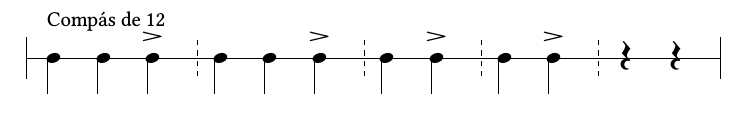
\includegraphics{figures/ud-03/ciclos-1.png}
\caption{Compás flamenco de 12}
\end{figure}

\hypertarget{os-modos-ruxedtmicos-medievais}{%
\subsubsection*{Os modos rítmicos medievais}\label{os-modos-ruxedtmicos-medievais}}
\addcontentsline{toc}{subsubsection}{Os modos rítmicos medievais}

Nos tratados medievais sobre música, xunto ao ritmo e á melodía (que habitualmente denominaban \emph{harmonía}), incluíase a \textbf{métrica} isto é, a organización sonora das palabras propia da poesía; debido a que a música era maioritariamente vocal, e o ritmo dependía desa organización.

No século XIII estableceuse unha organización rítmica baseada en modos, do mesmo xeito que a organización melódica. Estes modos derivaban dos pés métricos da poesía latina e eran seis:

\begin{figure}
\centering
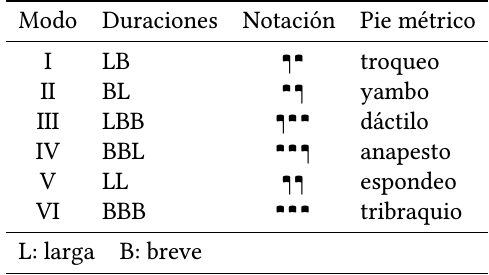
\includegraphics{figures/ud-03/modosritmicos.png}
\caption{Modos rítmicos}
\end{figure}

\hypertarget{o-sistema-modal-medieval}{%
\section*{O sistema modal medieval}\label{o-sistema-modal-medieval}}
\addcontentsline{toc}{section}{O sistema modal medieval}

Os primeiros libros de teoría musical do Occidente europeo corresponden ao século IX; entre eles destacan os dous tratados anónimos titulados \emph{Musica enchiriadis} («Manual de música») e \emph{Scolica enchiriadis} («Comentarios ao manual»), a partir dos cales se desenvólve unha importante corrente de literatura técnica musical, que explica o sistema sobre o que se compón a música monódica da Idade Media.

\hypertarget{as-especies-de-intervalos}{%
\subsection*{\texorpdfstring{As \emph{especies} de intervalos}{As especies de intervalos}}\label{as-especies-de-intervalos}}
\addcontentsline{toc}{subsection}{As \emph{especies} de intervalos}

O sistema modal medieval parte da \textbf{modalidade}, e tomaba como referencia os intervalos básicos de quinta e cuarta, así como a oitava. Os teóricos medievais partían das distintas \textbf{especies} destes intervalos, diferenciadas pola posición que ocupaba o semitono, como se pode ver na figura X.

\begin{figure}
\centering
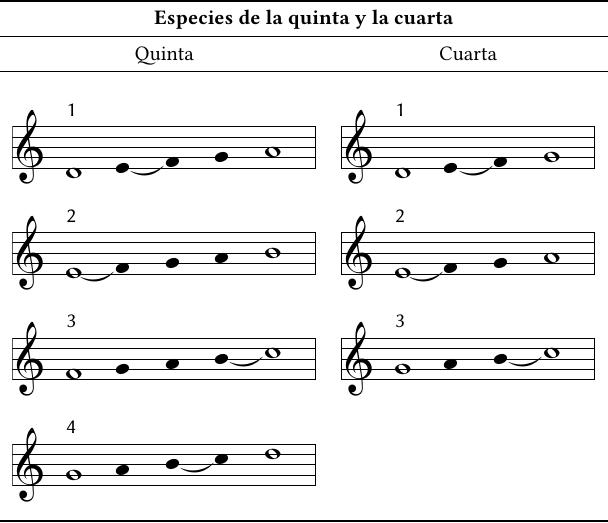
\includegraphics{figures/ud-03/especies.jpg}
\caption{Especies de quinta e cuarta}
\end{figure}

\hypertarget{os-modos-medievais}{%
\subsection*{Os modos medievais}\label{os-modos-medievais}}
\addcontentsline{toc}{subsection}{Os modos medievais}

As catro especies de quinta, son a base dos \textbf{catro modos básicos} da música medieval:

\begin{enumerate}
\def\labelenumi{\arabic{enumi}.}
\tightlist
\item
  \emph{protus} («primeiro»)
\item
  \emph{deuterus} («segundo»)
\item
  \emph{tritus} («terceiro»)
\item
  \emph{tetrardus} («cuarto»)
\end{enumerate}

Algúns teóricos, aplicaron os nomes da antiga teoría musical grega (con significado distinto) a estas catro especies da quinta, resultando: \emph{dórico}, \emph{frigio}, \emph{lidio} , \emph{mixolidio}.

Combinando cada especie de quinta cunha de cuarta, obtemos o que se coñece como modo. Segundo a súa combinación, podemos falar de \textbf{modos \emph{auténticos}} (se a especie de cuarta vai despois da de quinta), ou \textbf{modos \emph{plagales}} (se a especie de cuarta vai antes da especie de quinta). Para diferenciar os plagales dos anténticos, antepoñemos o prefixo \emph{hipo-} ao nome grego correspondente (\emph{hipo-}dórico, \emph{hipo}-frixio, \ldots{} ) tal como se indica na táboa do sistema modal medieval.

O sistema completo quedaba entón da forma:

\begin{figure}
\centering
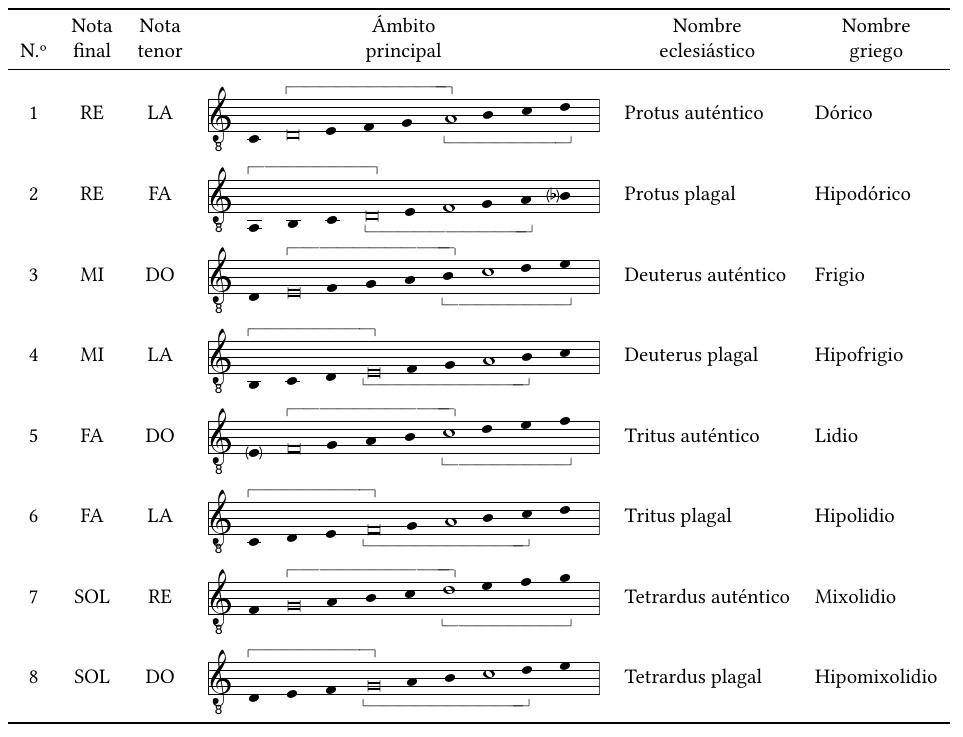
\includegraphics{figures/ud-03/sistema-modal.jpg}
\caption{Sistema modal}
\end{figure}

Se ben é certo, que na práctica o máis habitual era referirse aos modos cos números do 1 ao 8, nos tratados teóricos empregábanse tanto a denominación eclesiástica como a grega.

\hypertarget{tenor-finalis-e-uxe1mbito-da-meloduxeda}{%
\subsection*{\texorpdfstring{\emph{Tenor}, \emph{Finalis} e ámbito da melodía}{Tenor, Finalis e ámbito da melodía}}\label{tenor-finalis-e-uxe1mbito-da-meloduxeda}}
\addcontentsline{toc}{subsection}{\emph{Tenor}, \emph{Finalis} e ámbito da melodía}

A melodía do canto, abarca o ámbito da oitava. Adoita utilizar unha interválica sinxela; graos conxuntos ou saltos de terceira e só ocasionalmente aparecen saltos de quinta ou de cuarta, normalmente só nos comezos de frase.

Unha das notas da melodía, era considerada como a nota principal do modo que se coñece co nome de \emph{final} (na que remata a melodía). Outras notas da melodía, servían de soporte --ou eixos melódicos-- sobre os que se move a melodía; no canto gregoriano unha destas notas toma especial importancia e recibe o nome de \emph{tenor} («soporte» en latín).

Para determinar o modo no sistema medieval, debemos considerar:

\begin{enumerate}
\def\labelenumi{\arabic{enumi}.}
\tightlist
\item
  A nota \textbf{final}, que determina en cal do catro modos básicos está a melodía.
\item
  O \textbf{ámbito}, por encima da final no caso dos modos auténticos e ao redor dela nos plagales.
\item
  A nota \textbf{tenor} e outras que puidesen servir para as cadencias.
\item
  O uso de certos \textbf{xiros melódicos} característicos (incluídas as cadencias).
\end{enumerate}

\hypertarget{o-estilo}{%
\subsection*{O estilo}\label{o-estilo}}
\addcontentsline{toc}{subsection}{O estilo}

O estilo dunha peza viña determinado --ademais de polo modo-- por outros elementos tales como a relación entre melodía e texto, que daba lugar a dous estilos principais:

\begin{enumerate}
\def\labelenumi{\arabic{enumi}.}
\tightlist
\item
  \textbf{Estilo silábico}: a cada sílaba do texto correspóndelle unha nota ou como máximo dúas.
\item
  \textbf{Estilo ornamentado}: algunhas sílabas do texto, prolónganse con varias notas denominadas \emph{melismas}.
\end{enumerate}

Aínda que cada modo destaca certas notas e ten un ámbito determinado, teremos en conta que non se trata de alturas reais, senón de intervalos isto é; calquera modo podía cantarse transportado a calquera altura, sempre que se respectase a distribución dos intervalos.

\hypertarget{a-escrita}{%
\subsection*{A escrita}\label{a-escrita}}
\addcontentsline{toc}{subsection}{A escrita}

En principio, o sistema completo abarcaba dúas oitavas. Na escrita, utilizáronse as letras do alfabeto latino para designar as notas en orde ascendente. Co tempo, o sistema foise ampliando ata abarcar algo máis de dúas oitavas, diferenciadas polo uso de maiúsculas e minúsculas ou pola duplicación das letras.

O \emph{si} era unha nota de afinación variable: para evitar o tritono co fa podíase rebaixar medio ton, converténdoo así nun «si suave» (en latín \emph{b molle}), que se escribía cunha «b» redonda para diferencialo do «si duro» (\emph{b durum}) que se escribía cunha «b» cadrada (\emph{b quadratum}); estes signos son os antecedentes dos actuais \emph{bemol}, \emph{becuadro} e \emph{sostido}.

\begin{figure}
\centering
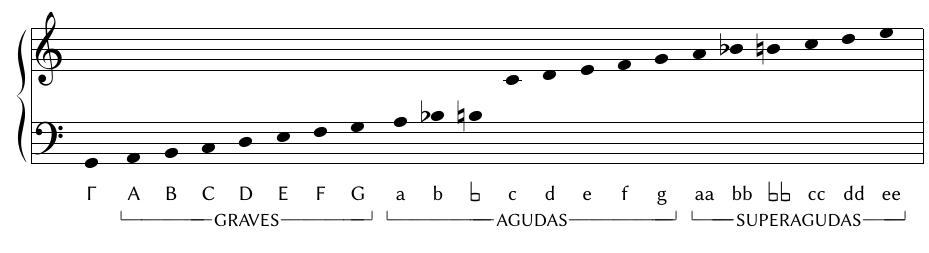
\includegraphics{figures/ud-03/sistemaCompleto.jpg}
\caption{Sistema completo}
\end{figure}

No século XI, o monxe e mestre de coro italiano \textbf{Guido d'Arezzo}, para facilitar a aprendizaxe das melodías, que seguían memorizándose, inventou un sistema que asociaba determinadas sílabas con notas e as súas combinacións con intervalos; para iso utilizou seis sílabas sacadas do texto dun himno relixioso: \emph{ut re mi fa sol la}. Nesta sucesión de seis sílabas todos os intervalos eran dun tono excepto o intervalo central \emph{mi-fa}, que era dun semitono.

A serie podía comezar na nota \emph{dó}, na nota \emph{fa} co «\emph{si} suave» e na nota \emph{sol} co «\emph{si} duro», resultando así o tres tipos \textbf{de hexacordos}:

\begin{figure}
\centering
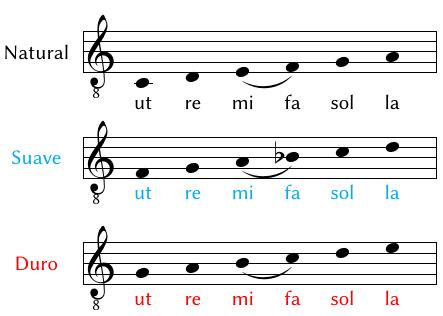
\includegraphics{figures/ud-03/hexacordos.jpg}
\caption{Os hexacordos}
\end{figure}

Posto que os hexacordos podían comezar en notas diferentes, en melodías máis amplas utilizábase un sistema de paso dun hexacordo a outro chamado \textbf{solmisación}.

\hypertarget{a-notaciuxf3n-musical-medieval}{%
\section*{A notación musical medieval}\label{a-notaciuxf3n-musical-medieval}}
\addcontentsline{toc}{section}{A notación musical medieval}

\hypertarget{a-notaciuxf3n}{%
\subsection*{A notación}\label{a-notaciuxf3n}}
\addcontentsline{toc}{subsection}{A notación}

Durante toda a Idade Media ---e mesmo despois--- a música seguiría transmitíndose oralmente. No século IX, en varios mosteiros de Occidente, desenvolveríase un sistema de escritura musical novo, que evolucionaría ao longo dos séculos ata desembocar no sistema actual. A principal razón deste desenvolvemento, foi a implantación do repertorio de canto chamado «gregoriano», pero non a única. Pretendíase tamén unificar a interpretación musical litúrxica en todos os territorios que dependían da Igrexa de Roma.

\hypertarget{os-neumas}{%
\subsubsection*{Os neumas}\label{os-neumas}}
\addcontentsline{toc}{subsubsection}{Os neumas}

As notacións máis antigas utilizaban uns signos chamados \textbf{neumas} que se escribían sobre as liñas do propio texto que se debía cantar. Estes neumas «debuxaban» o perfil melódico do canto, pero non con precisión a melodía que se aprendía por escoita e memorización.

Este primeiro sistema de notación presentaba numerosas variantes, dependendo do lugar (mosteiro ou rexión) en que se elaboraba cada manuscrito. Algunhas destas variantes, as chamadas \textbf{adiastemáticas}, centrábanse nas calidades da interpretación sen atender á interválica; outras, as chamadas \textbf{diastemáticas}, utilizaban diversos sistemas (puntos, liñas\ldots) para tratar de indicar a amplitude relativa dos intervalos.

Na primeira metade do século XI, \textbf{Guido d'Arezzo} reuniu varias técnicas que facilitaban a lectura a primeira vista e por tanto a aprendizaxe dos cantos; as principais características da súa proposta eran as seguintes:

\begin{itemize}
\tightlist
\item
  Os neumas situábanse sobre unha pauta de liñas \textbf{paralelas} que marcaban a distancia dunha terceira, e a lonxitude dos seus trazos indicaba a amplitude do intervalo.
\item
  As notas contiguas aos semitonos indicábanse con liñas de cores específicas: o \emph{fa} en cor vermella, o \emph{dó} en cor amarela.
\item
  Á esquerda desas liñas escribíanse \textbf{letras crave}, que indicaban esas mesmas notas: a \textbf{F} para o \emph{fa} e a \textbf{C} para o \emph{dó}.
\item
  Á dereita de cada pauta escribíase un pequeno signo, chamado \textbf{custos}, que indicaba a primeira nota da seguinte pauta e facilitaba así a entonación correcta do intervalo.
\end{itemize}

O \textbf{sistema guidoniano} tivo gran éxito e estendeuse inmediatamente por todo Occidente, aínda que as diversas notacións neumáticas seguíronse utilizando nalgúns lugares mesmo ata o século XVI.

Da notación guidoniana derivaron outras, como a notación alemá de cravo \textbf{de ferradura} ou a \textbf{notación cadrada} francesa, que naceu no século XII e que aínda se utiliza nos libros de canto gregoriano. Esta última adaptouse posteriormente para as cancións trovadorescas e outros xéneros de música profana. A partir do século XIII, as novas técnicas da música polifónica farán evolucionar a notacións, especialmente no aspecto rítmico.

\newpage

\hypertarget{consideraciuxf3ns-sobre-o-canto-gregoriano}{%
\section*{Consideracións sobre o Canto Gregoriano}\label{consideraciuxf3ns-sobre-o-canto-gregoriano}}
\addcontentsline{toc}{section}{Consideracións sobre o Canto Gregoriano}

\hypertarget{caracteruxedsticas-que-definen-o-canto-gregoriano}{%
\subsection*{Características que definen o canto gregoriano}\label{caracteruxedsticas-que-definen-o-canto-gregoriano}}
\addcontentsline{toc}{subsection}{Características que definen o canto gregoriano}

O canto gregoriano, como todo o canto litúrxico medieval, presenta as seguintes características:

\begin{itemize}
\tightlist
\item
  É un \textbf{canto monódico}, é dicir, utilízase unha soa liña melódica tanto para o canto solista como para o canto a un tempo.
\item
  O \textbf{ritmo} é \textbf{flexible}, dependendo do texto que se canta; non hai compás nin pulso regular, e tanto o fraseo como a distribución de acentos axústanse ás necesidades de declamación do texto.
\item
  O \textbf{ámbito} non supera normalmente a \textbf{oitava} (excepto en cantos para solistas, que poden superala nunha cuarta ou quinta).
\item
  Está baseado no \textbf{sistema modal} e foi descrito e organizado por teóricos musicais case sempre do ámbito monástico.
\item
  A melodía móvese por graos \textbf{conxuntos} ou \textbf{saltos de terceira}; ocasionalmente aparecen saltos de cuarta ou quinta, normalmente nos comezos. Son inhabituais intervalos máis amplos.
\item
  O perfil melódico de cada canto organízase ao redor de dous eixos: a \textbf{nota final}, na que termina e con frecuencia tamén comeza o canto, e a chamada \textbf{nota tenor} («soporte» en latín), sobre a que se desenvolve a melodía. Esta nota está normalmente unha quinta sobre a final nos modos auténticos e unha terceira por baixo desta nos plagales, excepto cando recae sobre a nota \emph{si}, que se pasa ao do.
\end{itemize}

\hypertarget{estilos-de-canto}{%
\subsubsection*{Estilos de canto}\label{estilos-de-canto}}
\addcontentsline{toc}{subsubsection}{Estilos de canto}

Segundo a relación entre o texto e a melodía, desenvólvense tres estilos de canto:

\begin{itemize}
\tightlist
\item
  \textbf{Silábico:} é o estilo máis simple: a cada sílaba do texto correspóndenlle unha ou dúas notas.
\item
  \textbf{Neumático:} estilo adornado; a cada sílaba correspóndenlle varias notas (normalmente de dúas a seis).
\item
  \textbf{Melismático:} estilo moi adornado; algunhas sílabas teñen melismas extensos, ás veces de decenas de notas; no resto adoita predominar o estilo neumático.
\end{itemize}

Nun mesmo canto mestúranse varios estilos, pero un deles predomina e é o que caracteriza a ese canto.

\hypertarget{estilos-de-interpretaciuxf3n}{%
\subsubsection*{Estilos de interpretación}\label{estilos-de-interpretaciuxf3n}}
\addcontentsline{toc}{subsubsection}{Estilos de interpretación}

Hai tamén tres estilos de interpretación (chamados tamén estilos de salmodia):

\begin{itemize}
\tightlist
\item
  \textbf{Directa}: cántanse todos os versos (ou versículos) sen interrupción, por un coro ou máis frecuentemente un solista.
\item
  \textbf{Antifonal}: alternan dous coros (ou dous pequenos grupos de cantantes, máis exactamente) cantando os versos impares e pares ou ben versos e un refrán.
\item
  \textbf{Responsorial}: alternan un solista e un coro, normalmente cantando aquel os versos e este o refrán.
\end{itemize}

\hypertarget{o-repertorio-do-canto-gregoriano}{%
\subsection*{O repertorio do canto gregoriano}\label{o-repertorio-do-canto-gregoriano}}
\addcontentsline{toc}{subsection}{O repertorio do canto gregoriano}

O repertorio gregoriano está formado fundamentalmente polos cantos que se interpretaban nas dúas grandes cerimonias litúrxicas: a misa e o oficio.

\hypertarget{cantos-da-misa}{%
\subsubsection*{Cantos da misa}\label{cantos-da-misa}}
\addcontentsline{toc}{subsubsection}{Cantos da misa}

Os cantos da misa dividíanse en dous grandes grupos: aqueles que se repetían a diario, durante todo o ano, ou en certas épocas chamados \textbf{cantos do ordinario}, interpretados polos asistentes; e aqueles que variaban en función da festa, do día ou da semana do ano litúrxico, chamados \textbf{cantos do propio}, cantados normalmente polas \emph{scholae} (coros profesionais).

\begin{itemize}
\item
  Os cantos do propio adóitanse clasificar en dous grupos:

  \begin{enumerate}
  \def\labelenumi{\arabic{enumi}.}
  \tightlist
  \item
    Antifonales (ou procesionais): cantados pola \emph{schola} durante cerimonias de duración variable; son o \textbf{introito}, o \textbf{ofertorio} e a \textbf{comunión}. Adoitan ser neumáticos e o ámbito móvese ao redor da oitava.
  \item
    Responsoriales (ou de meditación): cantados por solistas antes da lectura do evanxeo. Son o \textbf{gradual}, o \textbf{aleluia} e \textbf{o tracto}. Estes dous últimos eran excluíntes: cando se cantaba un non se cantaba o outro, en función da época do ano litúrxico. Todos son melismáticos e ás veces superan o ámbito da oitava.
  \end{enumerate}
\end{itemize}

Non debe confundirse este uso dos termos ``antifonal'' e ``responsorial'' cos estilos de interpretación citados antes.

\begin{itemize}
\item
  Os cantos do ordinario son cinco, que se coñecen polas palabras con que se inician os seus textos: \textbf{Kyrie}, \textbf{Gloria}, \textbf{Credo}, \textbf{Sanctus} e \textbf{Agnus Dei}.

  Son cantos moi antigos e na súa orixe eran cantados por tódolos asistentes. A partir do século XI compuxéronse centenares de melodías novas para eles, posiblemente porque xa non os cantaba a comunidade senón a \emph{schola}. Posteriormente serían tamén o núcleo principal na composición de misas polifónicas e concertadas.
\end{itemize}

\hypertarget{cantos-do-oficio}{%
\subsubsection*{Cantos do oficio}\label{cantos-do-oficio}}
\addcontentsline{toc}{subsubsection}{Cantos do oficio}

Entre tódalas obrigas das comunidades monásticas, atopábase a de reunirse para o rezo varias veces ao día; estes momentos denominábanse \emph{horas} e en conxunto constituían o \emph{oficio}. Desenvolvíase normalmente en oito sesións diarias, das que as máis importantes eran \textbf{vésperas} (na posta de sol), \textbf{maitines} (na medianoite) e \textbf{laudes} (coa saída do sol).

Se ben cada hora tiña unha estrutura diferente, os cantos do oficio pódense agrupar en varios tipos:

\begin{itemize}
\item
  \textbf{Salmos e cánticos}. Entoábanse mantendo a forma salmódica. A diferenza entre salmos e cánticos é litúrxica, segundo a procedencia do texto, pero musicalmente son semellantes.
\item
  \textbf{Antífonas}. Son o xénero máis numeroso do repertorio: eran cantos breves, de ámbito reducido, con intervalos melódicos pequenos, en estilo silábico, destinados ao canto por toda a comunidade. Cantábanse normalmente como introdución e conclusión dos salmos e cánticos.
\item
  \textbf{Responsorios}. Cantos de meditación, habitualmente en estilo melismático ou neumático e interpretados por solistas. Forman o segundo conxunto en cantidade despois das antífonas.
\item
  \textbf{Himnos}. Cantos estróficos, divididos habitualmente en estrofas de catro versos de oito sílabas, de igual melodía. Foron moi populares e existe un gran repertorio, malia non contar nos inicios coa aceptación das autoridades relixiosas, empregándose nunha parte marxinal da liturxia. Probablemente a súa popularidade puido deberse á súa semellanza cos cantos populares.
\end{itemize}

\hypertarget{autoruxeda-dos-cantos}{%
\subsection*{Autoría dos cantos}\label{autoruxeda-dos-cantos}}
\addcontentsline{toc}{subsection}{Autoría dos cantos}

A gran maioría das melodías do repertorio gregoriano e as dos seus predecesores son anónimas, en parte debido o escaso interese que os músicos medievais --e os artistas en xeral-- tiñan en canto á cuestión da autoría. Coñecemos varios nomes de compositores: entre eles, \textbf{Notker de San Gall} (s. IX-X), ou \textbf{Hildegard de Bingen} (s.XII) destacada escritora, científica e conselleira de papas e emperadores.

\hypertarget{expansiuxf3ns-do-canto-gregoriano}{%
\section*{Expansións do canto gregoriano}\label{expansiuxf3ns-do-canto-gregoriano}}
\addcontentsline{toc}{section}{Expansións do canto gregoriano}

Co paso do tempo, os músicos de igrexa continuaron creando música nova, que se engadía de diversas formas ás melodías gregorianas; desde pezas completamente novas, ben por novas festividades, ben para momentos que non tiñan cantos, como por exemplo as procesións. Neste último caso inclúense os cantos denominados \textbf{\emph{conductus}}.

De entre as técnicas e formas que aparecen neste contexto, destacan os \textbf{tropos}, as \textbf{secuencias} e os \textbf{dramas litúrxicos}.

\hypertarget{tropos}{%
\subsection*{Tropos}\label{tropos}}
\addcontentsline{toc}{subsection}{Tropos}

\emph{Tropo} designa actualmente un conxunto diverso de técnicas de ampliación dos cantos do repertorio gregoriano; na súa época, estas técnicas recibiron distintas denominacións.

Consiste en engadir música ou música e letra a un canto da misa ou do oficio. A súa práctica comeza en Francia no s. IX e difúndese rápidamente. É habitual no \href{https://open.spotify.com/track/0wTT2YyDjlqmjHe1HOIacE}{\emph{Kyrie}} e no \href{https://es.wikipedia.org/wiki/Benedicamus_domino}{\emph{Benedicamus Domino}}.

As técnicas de tropar son fundamentalmente tres:

\begin{itemize}
\item
  Adición de música. Consiste en engadir melismas a algunha ou algunhas das sílabas dun canto (con máis frecuencia, as últimas ou as primeiras). É a máis antiga e foi en orixe unha técnica de improvisación
\item
  Adición de texto: neste caso, non se engade un melisma senón texto nun canto, transformando este melisma nunha pasaxe en estilo silábico; recibía os nomes de prosa ou \emph{prosula}.
\item
  Adición de música e texto.

  É a técnica máis importante, e a que recibiu propiamente o nome de tropo . Consistía en engadir pasaxes breves (ás veces non tan breves) de texto con música, que se situaban ao comezo ou ao final dun canto, ou ben se intercalaban entre os versos de leste.
\end{itemize}

Como exemplo desta técnica atopamos o \emph{Kyrie fons bonitatis}, resultado de tropar con texto o \emph{Kyrie}:

\begin{figure}[ht]

{\centering 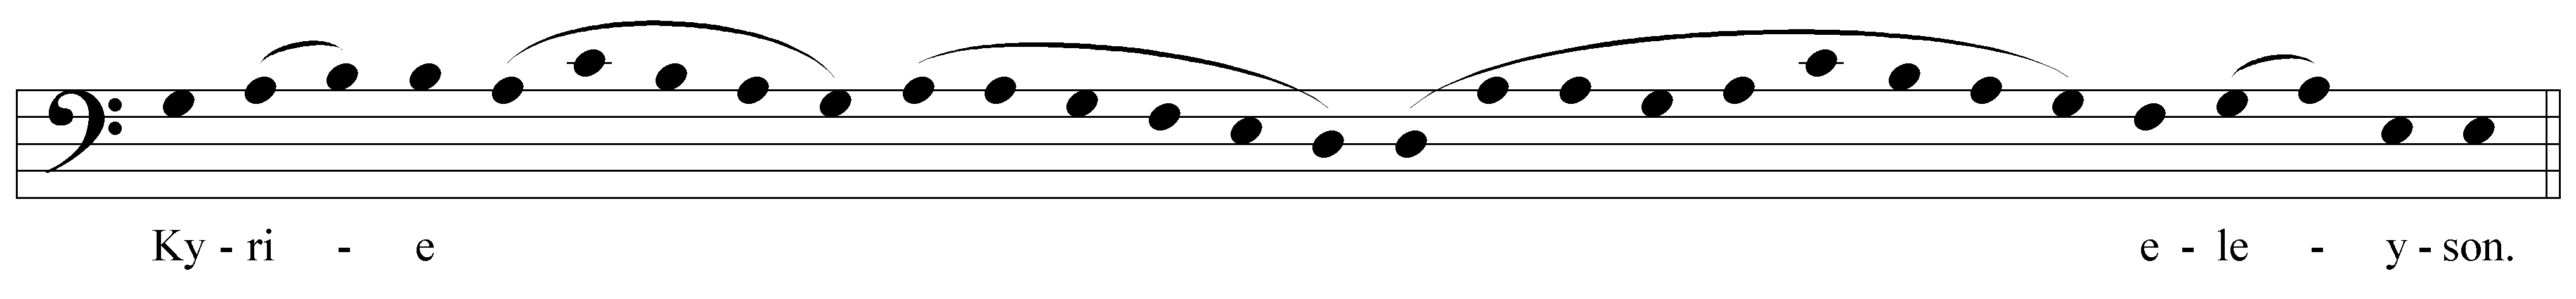
\includegraphics[width=1\linewidth]{figures/ud-03/Kyrie-1} 

}

\caption[Melodía do *Kyrie*]{Melodía orixinal do Kyrie}\label{fig:kyrie-1}
\end{figure}

A versión tropada, quedaría polo tanto do seguinte xeito no \href{https://es.wikipedia.org/wiki/Kyrie_eleison}{\emph{Kyrie fons bonitatis}}: \href{https://open.spotify.com/track/74ztOxzqhvEStzW4pqZII0?si=fbe1ed03f9bf4d6c}{(audición)}

\begin{figure}[ht]

{\centering 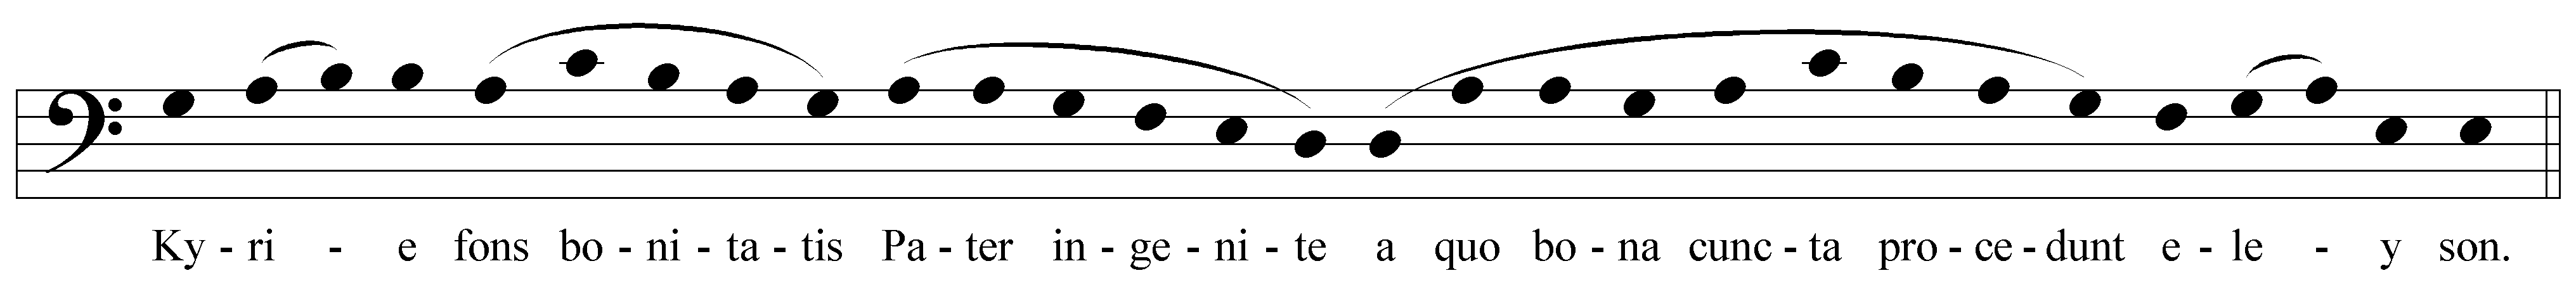
\includegraphics[width=1\linewidth]{figures/ud-03/Kyrie-fons-bonitatis} 

}

\caption[Melodía tropada do Kyrie fons bonitatis]{Melodía tropada do Kyrie}\label{fig:kyrie-fons-bonitatis}
\end{figure}

Os tropos tiveron un gran desenvolvemento desde o século IX ata o XVI, cando foron prohibidos polo concilio de Trento. Os cantos que se tropaban con máis frecuencia eran os cantos procesionais da misa (Introito, Ofertorio e Comunión) e os responsorios do oficio. Tamén se tropaban os cantos do ordinario da misa, a excepción do Credo.

\hypertarget{secuencias}{%
\subsection*{Secuencias}\label{secuencias}}
\addcontentsline{toc}{subsection}{Secuencias}

As secuencias son cantos independentes de nova composición que se interpretaban despois do aleluia na misa. A súa orixe puido estar relacionada cos tropos: en principio, a \emph{sequentia} aparece como un melisma engadido á última sílaba da palabra \emph{aleluia}; este melisma foi despois tropado e convertido en canto silábico, para finalmente independizarse completamente. Etimolóxicamente, \emph{sequentia} significa ``o que segue'' (melisma que segue ao aleluia).

As secuencias, son silábicas e consisten na repetición pareada: cada unidade melódica, repítese dúas veces con texto diferente antes de aparecer a seguinte, que pode ser totalmente distinta, salvo na primeira e última frase (a bb cc dd \ldots{} n). Esta sería a forma primitiva que recibe o nome de \textbf{forma de secuencia} e relaciónase con outras formas musicais da época, non só relixiosas.

A partir do século XIII o texto estrutúrase en estrofas co mesmo esquema métrico e rítmico, ben con unha mesma melodía ou alternando varias e recibe o nome de \textbf{forma estrófica}.

Do mesmo xeito que os tropos, as secuencias foron prohibidas polo concilio de Trento, agás as seguintes:

\begin{itemize}
\tightlist
\item
  \emph{Victimae paschali laudes} (Pascua)
\item
  \emph{Veni Sancte Spiritus} (Pentecostés)
\item
  \emph{Lauda Sion} (Corpus Christi)
\item
  \href{https://gl.wikipedia.org/wiki/Dies_irae}{\emph{Dies Irae}} (Misa de defuntos) \href{https://open.spotify.com/track/7IDZBDMZEkVzqHx3gpQ9yj?si=ca6c04c67bbc4f23}{(audición)}
\end{itemize}

Un dos exemplos máis coñecidos de \emph{sequentia} é o \emph{Dies irae (Officium defunctorum)} da misa de defuntos.

\begin{figure}[ht]

{\centering 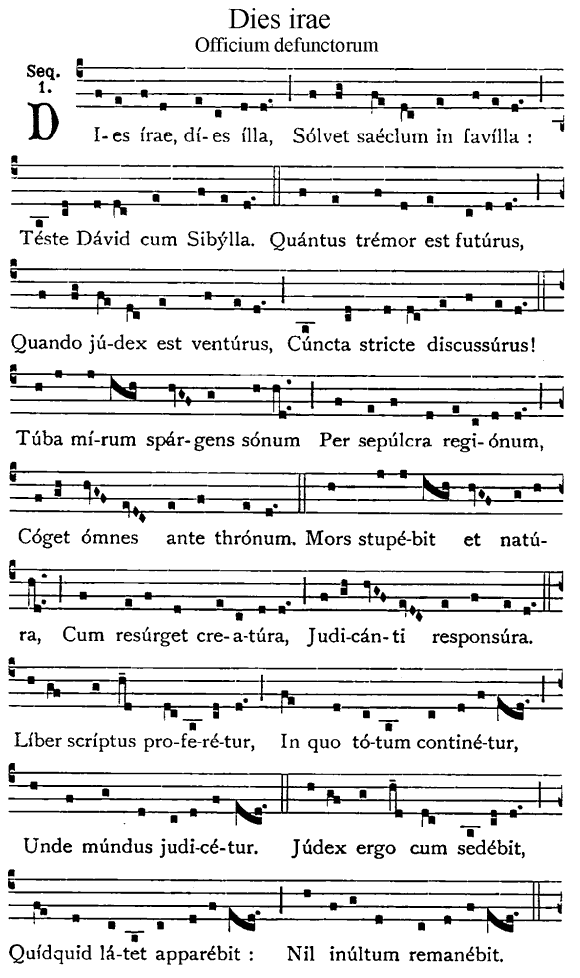
\includegraphics[width=0.75\linewidth]{figures/ud-03/Dies-irae} 

}

\caption[Secuencia Dies irae]{Exemplo da secuencia Dies Irae}\label{fig:Dies-irae}
\end{figure}

\hypertarget{o-drama-lituxfarxico}{%
\subsection*{O drama litúrxico}\label{o-drama-lituxfarxico}}
\addcontentsline{toc}{subsection}{O drama litúrxico}

O que coñecemos actualmente como \emph{drama litúrxico} é un tipo de composición dialogada, cantada na súa totalidade, que se representaba durante algunha cerimonia relixiosa en forma teatral. Datan de entre os séculos X e XVI; son dramas relixiosos en latín, que se representan nos tempos litúrxicos de Nadal e Semana Santa e probablemente a súa orixe proceda do desarrollo dramático de tropos dialogados.

A orixe do drama litúrxico adóitase relacionar cunha composición coñecida como \emph{Quem quaeritis}. Trátase dun breve diálogo entre uns anxos e as mulleres que buscan a Cristo no sepulcro o día de Resurrección. Nesta representación, o texto interpretábase por dous grupos de cantores que alternaban, representando os papeis de anxos e mulleres. \emph{Quem quaeritis} foi un referente do drama litúrxico; entre os séculos XII e XIII, comeza un importante auxe de obras musicais dialogadas e representadas, que incorporan historias bíblicas ou alegóricas, con multitude de personaxes e de extensión considerable. O \emph{Ludus Danielis} (s.XII) é un exemplo, onde por primeira vez aparecen escenas colectivas nas que se entoan gran cantidade de melodías, a maioría imitacións do canto gregoriano e dos tropos, así com secuencias. \emph{Ordo virtutum}, de \textbf{Hildegard de Bingen}, compositora e escritora do século XII, é outro exemplo. Como xénero non litúrxico, é máis probable que se admitise o uso de instrumentos como forma de aproximar aos fieles, os misterios das \emph{Sagradas Escrituras}.

\newpage

\hypertarget{actividades-e-audiciuxf3ns-desta-unidade}{%
\section*{Actividades e audicións desta unidade}\label{actividades-e-audiciuxf3ns-desta-unidade}}
\addcontentsline{toc}{section}{Actividades e audicións desta unidade}

\hypertarget{listado-de-audiciuxf3ns}{%
\subsection*{Listado de audicións}\label{listado-de-audiciuxf3ns}}
\addcontentsline{toc}{subsection}{Listado de audicións}

\hypertarget{anuxe1lise-e-comentario-de-audiciuxf3n-con-partitura}{%
\subsection*{Análise e comentario de audición con partitura}\label{anuxe1lise-e-comentario-de-audiciuxf3n-con-partitura}}
\addcontentsline{toc}{subsection}{Análise e comentario de audición con partitura}

Para realizar unha análise da obra, primeiramente faremos unha lectura a vista da información que nos ofrece; ollaremos a escrita prestando especial atención a tódolos elementos que observamos, tratando de identificalos. Dado que se trata dunha análise de audición con partitura, escoitaremos de seguido a obra tomando como guía a partitura, observando o perfil melódico, pausas, relación música texto, etc.

Trátase de realizar unha escoita activa da obra, prestando atención a tódolos elementos que nos permitan obter a máxima información posible para determinar o modo, o ámbito, estilo e forma, para finalmente clasificar a obra dentro do repertorio.

Debemos determinar:

\begin{enumerate}
\def\labelenumi{\arabic{enumi}.}
\tightlist
\item
  \textbf{modo} ao que pertence o canto
\item
  \textbf{ámbito} total da melodía
\item
  \textbf{estilo} de canto segundo ornamentación
\item
  \textbf{forma} ou estrutura formal
\item
  \textbf{clasificación} no repertorio
\end{enumerate}

\begin{center}\rule{0.5\linewidth}{0.5pt}\end{center}

\newpage

\hypertarget{audiciuxf3n-comentada-do-introito-puer-nuxe1tus-est-nuxf3bis}{%
\subsubsection*{\texorpdfstring{Audición comentada do Introito ``\emph{Puer nátus est nóbis}''}{Audición comentada do Introito ``Puer nátus est nóbis''}}\label{audiciuxf3n-comentada-do-introito-puer-nuxe1tus-est-nuxf3bis}}
\addcontentsline{toc}{subsubsection}{Audición comentada do Introito ``\emph{Puer nátus est nóbis}''}

\vspace*{0.25cm}

Realizaremos a análise e comentario da audición, prestando atención á partitura e os elementos que observamos na mesma.

\par
\vspace*{0.35cm}

\begin{figure}[ht]

{\centering 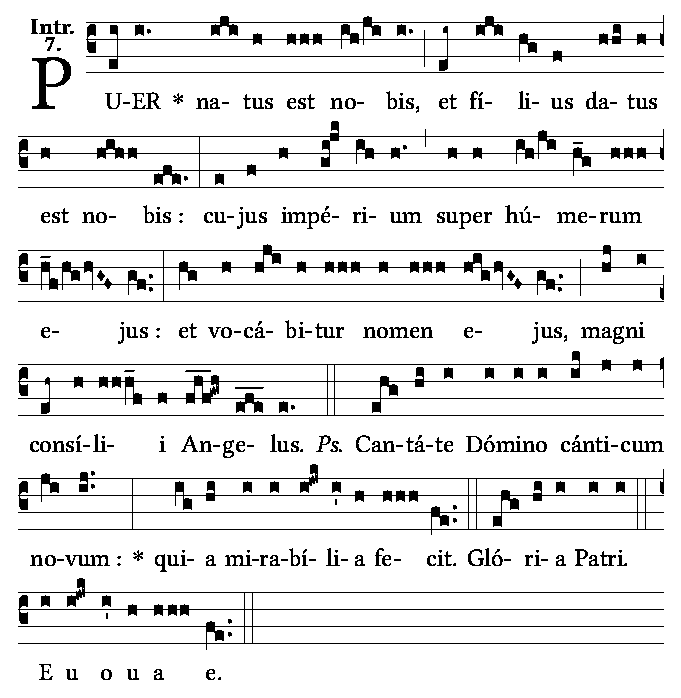
\includegraphics[width=1\linewidth]{figures/audicions/Puer-natus} 

}

\caption[Puer natus est  nobis]{Introito do Puer natus est nobis}\label{fig:Puer-natus-est}
\end{figure}

\begin{center}\rule{0.5\linewidth}{0.5pt}\end{center}

Se atendemos a unha primeira escoita da obra e tendo en conta a fonte de información facilitada, podemos deducir o seguinte:

\begin{enumerate}
\def\labelenumi{\arabic{enumi}.}
\item
  \textbf{Ritmo}. Estamos ante un tipo de ritmo \emph{non mensural} dado que non atende a pulso regular; neste caso axústase ao texto. Non se indica compás e carece de indicacións dinámicas; podemos afirmar que desenvolve o tempo natural da declamación. Algunhas notas, aumentan a súa duración nas sílabas do final de frase e inciso, atendendo aos \emph{punctum mora vocis}, que coinciden cos signos de puntuación do texto.
\item
  \textbf{Melodía}. En canto ao tipo de melodía, observamos un salto de quinta na primeira sílaba; as notas non presentan grandes saltos, discurrindo por graos conxuntos con excepción de saltos de terceira tanto ascendentes como descendentes. Trátase dunha melodía diatónica.

  \begin{itemize}
  \tightlist
  \item
    \textbf{Modo}: a nota final da peza é un \emph{sol} no primeiro espazo en clave de \emph{dó en terceira}. O modo básico por tanto, debe ser \emph{tetrardus} (IV). A nota máis aguda é un \emph{fa} que está unha sétima por encima da final; a nota máis grave (o \emph{sol}) é a mesma que a nota final. O modo é por tanto \emph{tetrardus auténtico}, que corresponde co número 7. O tenor, que pode verse ao comezo da cadencia de \emph{salmo} sobre o ``E'', é \emph{re} (dominante de \emph{sol}) que corresponde coa nota tenor do modo 7.\\
  \item
    \textbf{Ámbito}: o ámbito total abarca desde o nota final \emph{sol} ata o \emph{fa}, unha sétima que é un ámbito próximo á oitava pero inferior a ela; polo tanto, é un ámbito máis ben pequeno.\\
  \item
    \textbf{Estilo de canto}: tendo en conta que se cantan a maioría das sílabas adornadas cun \emph{neuma} de entre dúas e sete notas, estamos ante un estilo de canto neumático. A segunda sección, ao tratarse dun verso de \emph{salmo}, ten un estilo máis \emph{silábico}.
  \end{itemize}
\item
  \textbf{Timbre}. Polas características da obra e a audición da mesma, diferenciamos un coro de voces masculinas cantando \emph{a capella}, sen ningún tipo de acompañamento instrumental.
\item
  \textbf{Textura}. Percíbese na audición, unha pequena reverberación que provoca un efecto \emph{sostenuto} dalgunhas notas mentres soan as seguintes a modo de solape, creando así un efecto harmónico que non debemos confundir na textura. Trátase pois, dunha textura melódica de escrita horizontal onde só hai unha única liña melódica que todos cantan ao unísono; obedece a unha textura monódica.
\item
  \textbf{Forma} ou estrutura formal. A peza comeza cunha sección extensa (A) que chega ata a primeira dobre barra no cuarto \emph{tetragrama}. De seguido cántase un verso de salmo (B) seguido da \emph{doxoloxía} (C) cantada coa mesma melodía do \emph{salmo} e que aparece abreviada só co comezo (\emph{Gloria Patri}) e o final (\emph{seculorum amen}, escrito \emph{Euouae}). A continuación, volve ao comezo e cántase ata o final da sección A, polo que a forma completa sería ABCA. Estamos ante unha forma de estrutura ternaria de ``Canto Gregoriano''
\item
  \textbf{Clasificación} no repertorio. Tendo en conta o \textbf{ámbito} de sétima e o \textbf{estilo} neumático do canto, a peza debía ser interpretada polos cantores profesionais e por tanto debe ser un canto \emph{antifonal} do \emph{propio} da misa. A estrutura formal, coa inclusión de versos de \emph{salmo}, corresponde tamén a este tipo de cantos.
\end{enumerate}

Con todos estes datos, estamos en disposición de elaborar a ficha de audición correspondente, onde indicaremos o título da obra, autor, xénero, estilo, etc.

\begin{enumerate}
\def\labelenumi{\arabic{enumi}.}
\setcounter{enumi}{6}
\tightlist
\item
  Datos da obra
  Título da obra: \emph{Puer natus est nobis}
  Autor: anónimo
  Xénero: Vocal relixioso
  Estilo: Canto chá
\end{enumerate}

\hypertarget{exemplo-no.2-gradual-viduxe9runt-uxf3mnes}{%
\subsubsection*{\texorpdfstring{Exemplo no.2: Gradual ``\emph{Vidérunt ómnes}''}{Exemplo no.2: Gradual ``Vidérunt ómnes''}}\label{exemplo-no.2-gradual-viduxe9runt-uxf3mnes}}
\addcontentsline{toc}{subsubsection}{Exemplo no.2: Gradual ``\emph{Vidérunt ómnes}''}

O exemplo da figura \ref{fig:Puer-natus-est}, pertence ao Gradual ``\emph{Vidérunt ómnes}''.

\begin{figure}[h]

{\centering 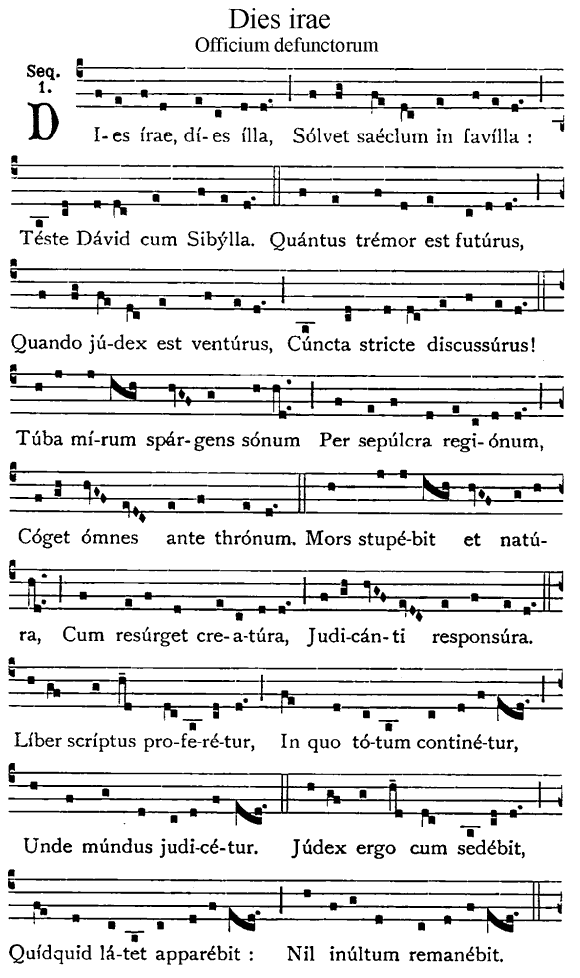
\includegraphics[width=1\linewidth]{figures/ud-03/Dies-irae} 

}

\caption[Vidérunt ómnes]{Fragmento do Gradual Vidérunt ómnes}\label{fig:Viderunt-omnes}
\end{figure}

%%%%% REFERENCES

% JEM: Quote for the top of references (just like a chapter quote if you're using them).  Comment to skip.
% \begin{savequote}[8cm]
% The first kind of intellectual and artistic personality belongs to the hedgehogs, the second to the foxes \dots
%   \qauthor{--- Sir Isaiah Berlin \cite{berlin_hedgehog_2013}}
% \end{savequote}

\setlength{\baselineskip}{0pt} % JEM: Single-space References

{\renewcommand*\MakeUppercase[1]{#1}%
\printbibliography[heading=bibintoc,title={\bibtitle}]}

\end{document}
